\documentclass[11pt,a4paper]{article}
\usepackage[margin=2.2cm]{geometry}
\usepackage{graphicx}
\usepackage{booktabs}
\usepackage{hyperref}
\usepackage{tikz}
\usetikzlibrary{shapes.geometric,arrows.meta,positioning,fit,backgrounds}
\usepackage{listings}
\usepackage{xcolor}

\begin{document}
\begin{titlepage}
\centering
\vspace*{1.5cm}
{\Large\bfseries Khulna University of Engineering and Technology\par}
\vspace{0.3cm}
{\large Department of Computer Science and Engineering\par}
\vspace{2.5cm}
{\huge\bfseries AES-128 Transparent Memory\\[4pt] Encryption on FPGA\par}
\vspace{0.6cm}
{\large Hardware Implementation Report\par}
{\normalsize Digilent Basys~3 (Artix-7 XC7A35T)\par}
\vspace{2.0cm}
{\large\bfseries Course:} Digital Signal Design\quad(\textbf{No:} 4224)\\[1.2cm]

\begin{minipage}{0.45\textwidth}
\begin{flushleft}\large
\textbf{Submitted to:}\\[4pt]
Md.\ Shakhawat Hossain\\
\textit{Assistant Professor}\\[6pt]
Dr.\ Muhammad Aminul Haque\\
\end{flushleft}
\end{minipage}
\hfill
\begin{minipage}{0.45\textwidth}
\begin{flushright}\large
\textbf{Submitted by:}\\[4pt]
Meheru Zannat\\
Roll: 2007039\\[6pt]
Bishal Roy\\
Roll: 2007098
\end{flushright}
\end{minipage}

\vfill
{\large \today\par}
\end{titlepage}

\section{Objective}
Design and verify an AES-128 ECB image encryption/decryption pipeline on
the Basys~3 FPGA. A $128{\times}128$ grayscale image is streamed from a
host PC over UART, encrypted in hardware, stored in on-chip BRAM, and
decrypted on demand back to the PC.

\section{Introduction}
The system implements transparent memory encryption around the
\texttt{secworks} AES-128 core. Custom RTL handles UART framing, block
assembly, BRAM storage, and FSM sequencing. A Python host transfers
16{,}384~bytes (1024 blocks of 128~bits) at 115200~baud. Mode is
selected by \texttt{SW0}; decrypt readback is triggered by \texttt{btnR}.

\section{Theory}
\textbf{AES-128.} 10-round symmetric block cipher over a $4{\times}4$
byte state: \textit{SubBytes}, \textit{ShiftRows}, \textit{MixColumns},
\textit{AddRoundKey} (final round omits \textit{MixColumns}).
Key schedule expands the 128-bit key into eleven round keys; expansion
is performed once per session and cached in \texttt{aes\_key\_mem}.\\
\textbf{\texttt{aes\_core} handshake.} \texttt{init} pulse triggers key
expansion (\texttt{ready} falls then rises); \texttt{next} pulse
processes one block and emits \texttt{result} when \texttt{ready} rises
again. \texttt{aes\_ctrl} skips key expansion after the first block via
a \texttt{key\_expanded} flag.\\
\textbf{UART.} 8N1 @ 115200, double-flop synchronizer, mid-bit
sampling.\\
\textbf{BRAM.} Inferred BRAM36 tile, 1024$\times$128~bit, synchronous
read/write.

\section{System Architecture}
Six custom modules wrap the \texttt{secworks} core. Signal connections
follow \texttt{top.v}.

\begin{figure}[h]
\centering
\begin{tikzpicture}[
  font=\footnotesize,
  node distance=1.6cm and 1.8cm,
  mod/.style={draw,thick,rounded corners,minimum width=2.4cm,
              minimum height=1.0cm,align=center,fill=blue!6},
  ext/.style={draw,thick,minimum width=1.6cm,minimum height=1.0cm,
              align=center,fill=gray!15},
  ctrl/.style={draw,thick,rounded corners,minimum width=2.4cm,
               minimum height=1.0cm,align=center,fill=orange!15},
  lbl/.style={font=\scriptsize,inner sep=1pt,fill=white},
  flow/.style={-{Latex[length=2mm]},thick}
]
\node[ext]                     (pc)   {PC\\(Python)};
\node[mod,right=of pc]         (rx)   {\texttt{uart\_rx}};
\node[mod,right=of rx]         (pb)   {\texttt{pixel\_buffer}};
\node[ctrl,right=of pb]        (aes)  {\texttt{aes\_ctrl}\\+\,\texttt{aes\_core}};
\node[ctrl,above=1.4cm of aes] (top)  {\texttt{top} FSM};
\node[mod,below=1.8cm of aes]  (bram) {\texttt{bram\_ctrl}\\1024$\times$128};
\node[mod,left=of bram]        (tx)   {\texttt{uart\_tx}};
\node[ext,left=of tx]          (pc2)  {PC\\(Python)};

\draw[flow] (pc) -- node[lbl,above]{serial} (rx);
\draw[flow] (rx) -- node[lbl,above]{\texttt{rx\_data}}
                    node[lbl,below]{\texttt{rx\_valid}} (pb);
\draw[flow] (pb) -- node[lbl,above]{\texttt{pbuf\_block}}
                    node[lbl,below]{\texttt{pbuf\_valid}} (aes);
\draw[flow] (aes) -- node[lbl,right]{\texttt{block\_out[127:0]}} (bram);
\draw[flow,dashed] (bram.east) -- ++(1.2,0)
      |- node[lbl,pos=0.25,right]{\texttt{bram\_dout}} (aes.east);
\draw[flow] (bram) -- node[lbl,above]{decrypt bytes} (tx);
\draw[flow] (tx)  -- node[lbl,above]{serial} (pc2);

\draw[flow,orange!70!black] (top) -- node[lbl,right]{\texttt{start,mode}} (aes);
\draw[flow,orange!70!black] (top.east) -| ++(1.0,-2.2)
      node[lbl,pos=0.25,above]{\texttt{wr/rd\_en,addr}} |- (bram.east);
\draw[flow,orange!70!black] (top.north) |- ++(-0.6,0.5) -|
      ($(tx.north)+(0,0.1)$)
      node[lbl,pos=0.25,above]{\texttt{tx\_data,send}};
\end{tikzpicture}
\caption{Module-level block diagram. Solid arrows: datapath
(encrypt flow left$\to$right). Dashed: decrypt readback from BRAM into
\texttt{aes\_ctrl}. Orange: control signals from \texttt{top} FSM.}
\end{figure}

\subsection{Module Interfaces}
\begin{itemize}\itemsep2pt
\item \texttt{uart\_rx}: \texttt{rx}$\to$\texttt{data\_out[7:0]},
      \texttt{data\_valid} (1-cycle pulse).
\item \texttt{pixel\_buffer}: gated by \texttt{rx\_valid \& \~{}mode\_sw};
      asserts \texttt{block\_valid} every 16 bytes (MSB-first pack).
\item \texttt{aes\_ctrl}: \texttt{key\_in[127:0]}, \texttt{block\_in},
      \texttt{mode} (1=enc, 0=dec), \texttt{start}$\to$
      \texttt{block\_out}, \texttt{done}. Drives \texttt{aes\_core}
      init/next handshake; caches key expansion.
\item \texttt{bram\_ctrl}: \texttt{wr\_en}, \texttt{rd\_en},
      \texttt{addr[9:0]}, \texttt{din[127:0]}, \texttt{dout[127:0]}.
\item \texttt{uart\_tx}: \texttt{data\_in[7:0]}, \texttt{send},
      \texttt{ready}$\to$\texttt{tx}.
\item \texttt{top}: 7-state FSM
      (\texttt{IDLE}, \texttt{ENC\_WAIT}, \texttt{ENC\_STORE},
      \texttt{DEC\_READ}, \texttt{DEC\_WAIT}, \texttt{DEC\_TX},
      \texttt{DONE}); maintains \texttt{wr\_addr}, \texttt{rd\_addr},
      \texttt{tx\_byte\_idx}, \texttt{encrypt\_done\_flag}.
\end{itemize}

\subsection{Specifications}
\begin{center}\small
\begin{tabular}{ll}\toprule
Board & Basys~3 / XC7A35T-1CPG236C \\
Clock & 100\,MHz \\
UART & 115200 8N1 \\
Cipher & AES-128 ECB (secworks core) \\
Image & 128$\times$128 grayscale, 16\,KB \\
Blocks & 1024 $\times$ 128\,bit \\
Storage & 1 $\times$ BRAM36 \\
Key & \texttt{2b7e151628aed2a6abf7158809cf4f3c} (FIPS-197) \\
\bottomrule
\end{tabular}
\end{center}

\section{Input / Output}
\begin{figure}[h]
\centering
\begin{tabular}{cc}
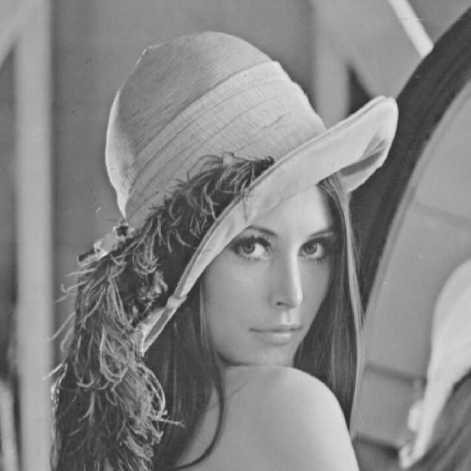
\includegraphics[width=5cm]{lena.png} &
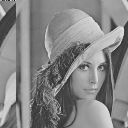
\includegraphics[width=5cm]{lena_decprepted.png}\\
(a) Input \texttt{lena.png} & (b) Decrypted output
\end{tabular}
\caption{End-to-end verification. Decrypted image is bit-identical to
input.}
\end{figure}

\section{Discussion}
The \texttt{aes\_ctrl} FSM correctly tracks the \texttt{ready} low/high
transitions of \texttt{aes\_core}, amortising key expansion across 1024
blocks. The critical path lies in the \texttt{aes\_sbox} pipeline;
post-implementation WNS at 100\,MHz is $\sim$3\,ns on Artix-7.

Throughput is UART-bound: at 115200~baud, 16\,KB requires
$\approx 1.4$\,s per direction, while \texttt{aes\_core} processes a
block in tens of cycles ($\approx 0.2\,\mu$s), two orders of magnitude
faster than the link. A USB-FIFO or Ethernet MAC would expose the
core's true throughput ($\sim$6\,Gbps theoretical).

ECB mode is used for simplicity; it leaks block-level spatial structure
and is unsuitable for production. CBC/CTR/GCM would require an IV path
and (for GCM) a GHASH unit. The key is hard-coded in \texttt{top.v};
real deployment requires secure key provisioning.

Resource usage is dominated by the S-Box LUT arrays; a single BRAM36
tile holds the entire ciphertext image, leaving the fabric largely
free.

\section{Conclusion}
A complete UART--AES--BRAM pipeline was implemented and verified on the
Basys~3. Bitwise-identical decryption of \texttt{lena.png} confirms
correct operation of all six custom modules and the \texttt{aes\_core}
handshake sequencing in \texttt{aes\_ctrl}. The design is a compact
baseline for future work on chained modes, authenticated encryption,
and higher-bandwidth host interfaces.

\section*{References}
\begin{enumerate}\itemsep1pt
\item NIST FIPS-197, \textit{Advanced Encryption Standard}, 2001.
\item J.\ Str\"ombergson, \texttt{secworks/aes} Verilog core,
      \url{https://github.com/secworks/aes}.
\item Digilent, \textit{Basys 3 Reference Manual}.
\item Xilinx UG473, \textit{7~Series Memory Resources}.
\item Xilinx, \textit{Vivado Design Suite User Guide}, 2023.1.
\end{enumerate}

\end{document}
